\subsection{Design Changes}
Some major changes were made to the specified design during a full rewrite of the code, this was mainly done to improve the readability and simplicity of the code, as well as making some large changes to the underlying structure of the code and the way that memory was managed. (Including object structure and the inclusion of polymorphism.)

\paragraph{}
The main force calculation algorithms were also modified to be much more efficient in terms of the extremely high memory usage. The end result was a definite performance improvement as well as lower memory usage.

\subsubsection{Program Structure Changes}
One of the largest changes that was made to the function of the program was to the body storage vectors, while previously they stored the actual body object, they now store only the pointer to a body object.

\paragraph{}
Bodies are now allocated to the vectors using dynamic memory allocation in order to prevent the objects from being deleted when they go out of scope, the disadvantage of this is that care must be taken to ensure that memory is freed correctly to prevent large memory leaks.

\paragraph{}
All control variables are now stored in an independent data structure, which is much simpler to keep track of from a code point of view, as all variables can be passed around in one go, leading to much tidier code. The type is defined in the scenario base class interface file but is independent of the scenario class itself. (The type is used in the scenario class.)

\paragraph{}
The scenario base class is now inherited by three subclasses; render, simulation, and shared, the base class contains virtual methods for passing the control and body pointer vector in and out of the individual objects, ensuring that a constant syntax is kept throughout the program for this management.

\paragraph{}
Because pointers are used in the body structure, copies must be made of the physical objects for render, simulation and shared, this is handled by the update methods themselves, the old objects are correctly freed from memory and new ones are dynamically allocated.

\paragraph{}
The methods are declared in the base class as virtual, the defaults will be inherited and used as is in the render and simulation classes, but they are overridden in the shared class to include mutex locking code, this prevents simultaneous access to the data through the shared object, ensuring data integrity and the correct operation of the program.

\paragraph{}
Some functions are present to allow quick access to variables inside the control structure, Paused and Exit status, these functions are also declared as virtual to allow them to be overridden in the shared class with similar mutex locking code.

\paragraph{}
In the shared class, because it now inherits the common scenario class it only contains a single buffer for control and body storage, once again simplifying the management of data flow. The mutex locks have also been greatly simplified, now only having a mutex for the body pointer storage and one for control.

\subsubsection{Algorithm Changes}
Algorithms that were modified where the calculation and summation of all forces, in essence, these algorithms are now combined into a single function, however the previous code focused around the use of a dynamic 2D vector matrix. The disadvantage of this is that the memory requirement is extremely high compared to what is required for the bodies themselves. 

\paragraph{}
The matrix was used for the storage of the X and Y forces for every single body relationship until they could be added together to get the final force on the bodies, the matrix had a type of double, meaning 8 bytes per item, with 1000 bodies, this represents 8MB of allocated memory, while bodies would only account for 280kB. (10000 bodies would use 800MB just for force storage and just 2.8MB for bodies themselves!)

\paragraph{}
While in the grand scheme of things, these amounts of memory are not going to make a dent in the system memory itself, I mainly made this change on principle that I wanted to design a system that would be easily scalable for any future changes that may make performance such that a large number of bodies is feasible to use. (Such as CUDA GPGPU Acceleration, 100000 bodies has an acceptable level of performance on a high end GPU using the brute force method. If the matrix was used, 80GB of memory would be needed for the force matrix and 28MB for bodies, at this point you can see how excessive this level of usage gets.)

\paragraph{}
The replacement of this method makes two major changes, first it removes any actual storage of the final force from the body object entirely, instead, the force is calculated for both bodies in a iterative for loop, acceleration is calculated for each body and added directly to the acceleration, all bodies are calculated and the acceleration is added on top for each relationship.

\paragraph{}
This results in an increase in performance mainly due to having fewer steps to the algorithm, a similar level of performance that was achieved at 1000 bodies on the previous code is now possible with 2000 bodies on the new code, which is a significant improvement.

\paragraph{}
Other than these changes, the code is fairly similar, some items have been moved around in order to reduce the overall number of source files present in the program.

\subsubsection{Time Constraints}
The main reason that the project was rewritten from scratch was to improve the readability and maintainability of the code, as well as making it easier to implement some critical features (adding and deleting bodies), which were causing crashes in the previous code.

\paragraph{}
Unfortunately due to this, time had to be taken away that would of been spent on certain features was taken up by this task. Features such as scenario saving and loading, are not present in the final code as time was used up.

\subsection{Object Orientation Changes}
The main change in program structure has been to object orientation, now with the inclusion of polymorphic methods for the shared area. The new structure is a simpler and a lot more logical than the previous which should allow more flexibility and clarity when it comes to maintenance and adding features.

\pagebreak
\subsubsection{Object Inheritance Diagram}
\begin{figure}[!ht]
  \centering
  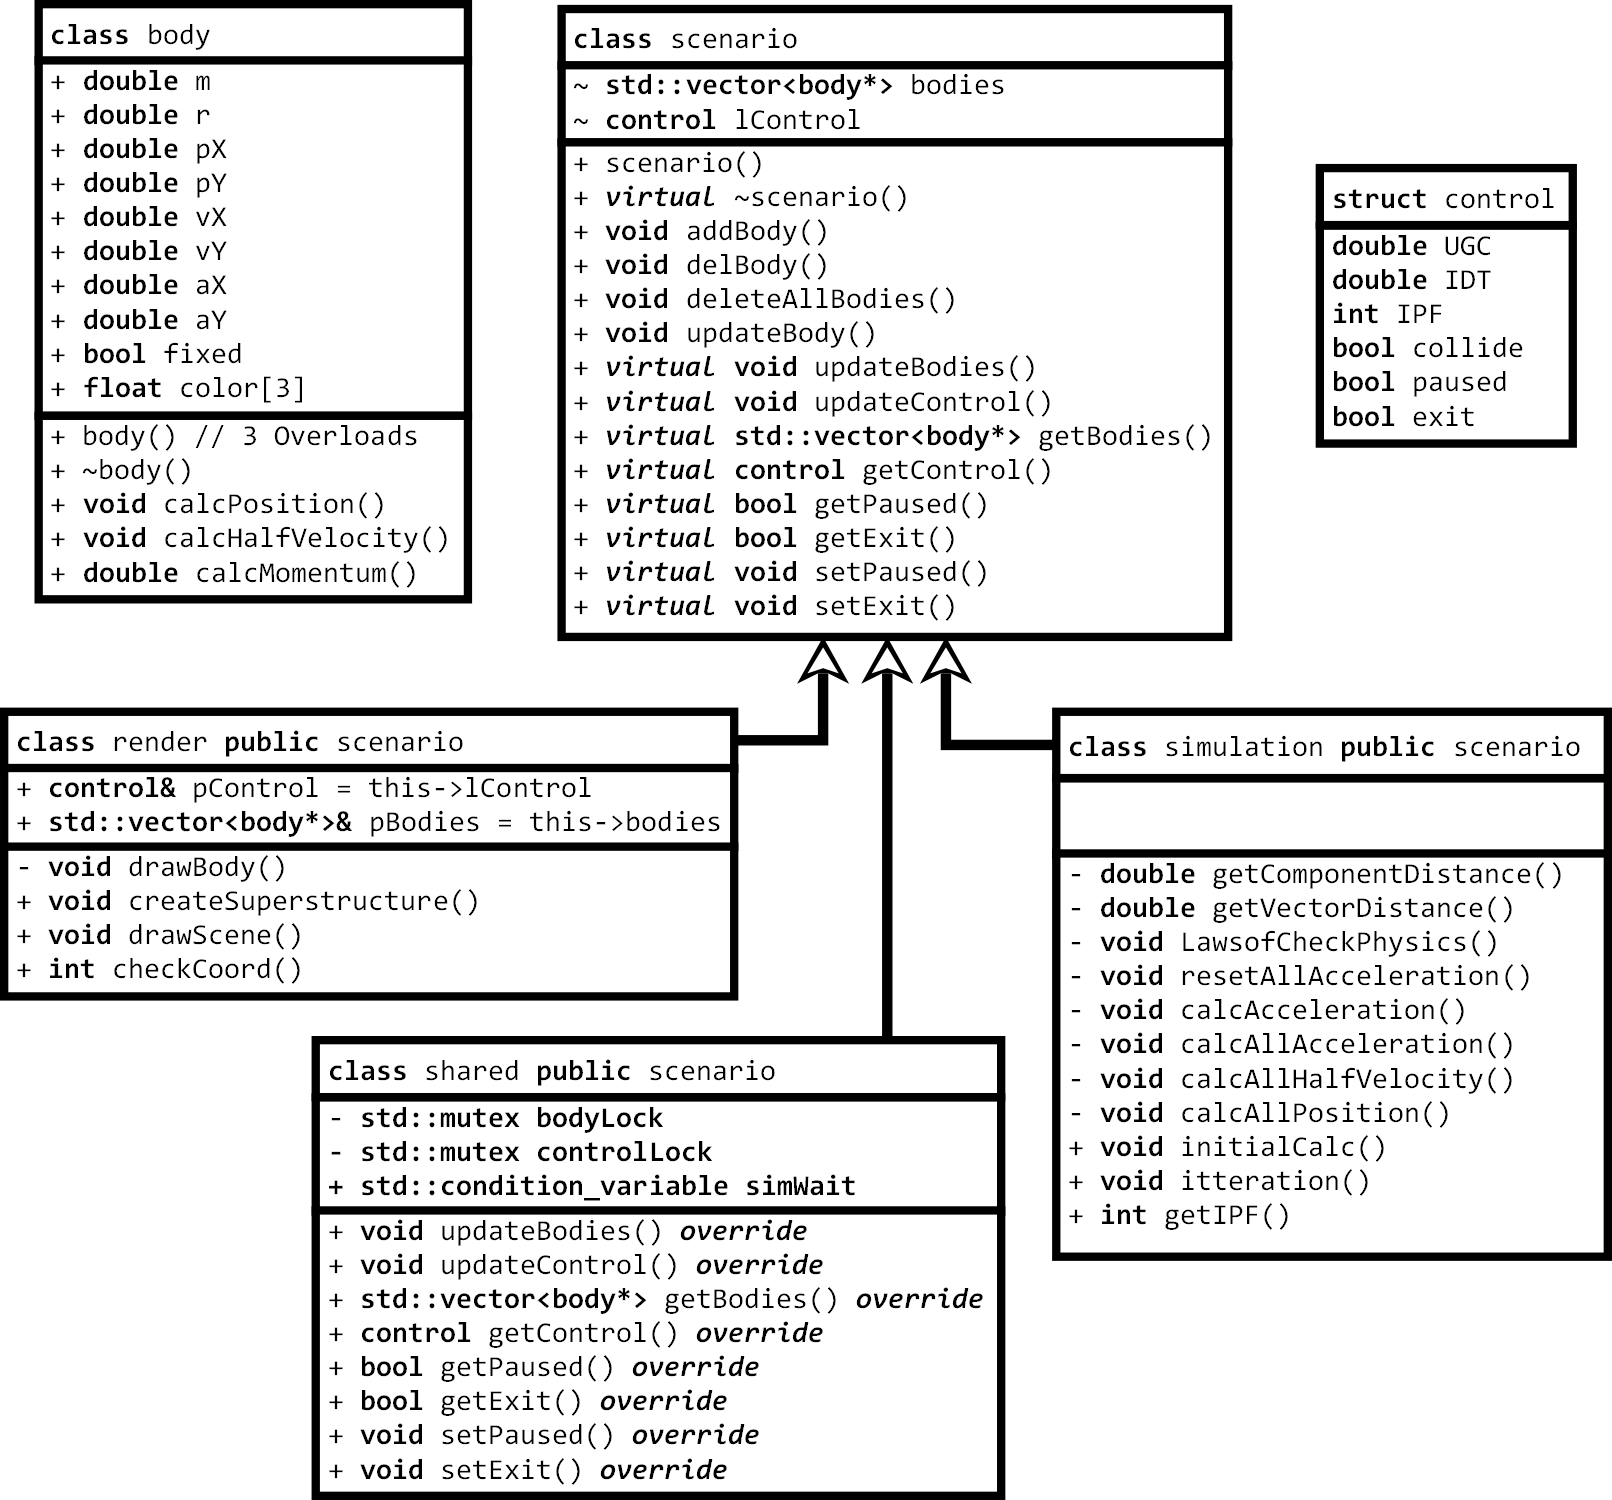
\includegraphics[width=\textwidth]{img/didredo.png}
  \caption{Improved Object Inheritance Diagram}
\end{figure}

\paragraph{}
Another notable change to the program structure is that the body object no longer makes use of encapsulation, the previous structure of the body class had all of the attributes in the body object fully encapsulated, however this just served to make the code more verbose and less clear, as well as causing difficulty when it came to the programming for the interface, as it requires direct access to variables and cannot access function calls.

\paragraph{}
The benefit to keeping the encapsulation in place was limited to non-existent, as no checking is being done in the actual body object itself, because of the amount of these objects it makes more sense to use them as a just a simple data structure which contains some calculation methods that apply to the individual objects.

\paragraph{}
The major focus of the code rewrite was to slim down the code in a way that improved its readability, memory usage and performance, an individual body object now only makes use of 77 bytes as opposed to 93, as force no longer has storage in the body object.

\paragraph{}
Another potential reduction that could be implemented is to change the data type of the colour storage, as it stands it is an array of three floats, this comes to 12 bytes. This figure could be reduce by using an array of 3 bytes variables to store the colour information. This would bring the total usage down to 68 bytes per object.

\paragraph{}
Further reductions could be made my switching to using single precision floating point variables for the simulation data storage, this would greatly reduce the accuracy of the simulation however. If colour, radius and fixed status were not required, the size could be brought down further to 28 bytes. At this point, there are not many options for further reductions in size and the feature set is greatly reduced. (More suited for a straightforward simulation rather than an interactive teaching example) In the case that GPU acceleration was implemented, single precision floating point would need to be used to take the best advantage of the hardware.

\pagebreak
\subsection{Flowchart Revision}
The flowchart has also underwent minor changes to better represent the new system that has been implemented.

\begin{figure}[!ht]
  \centering
  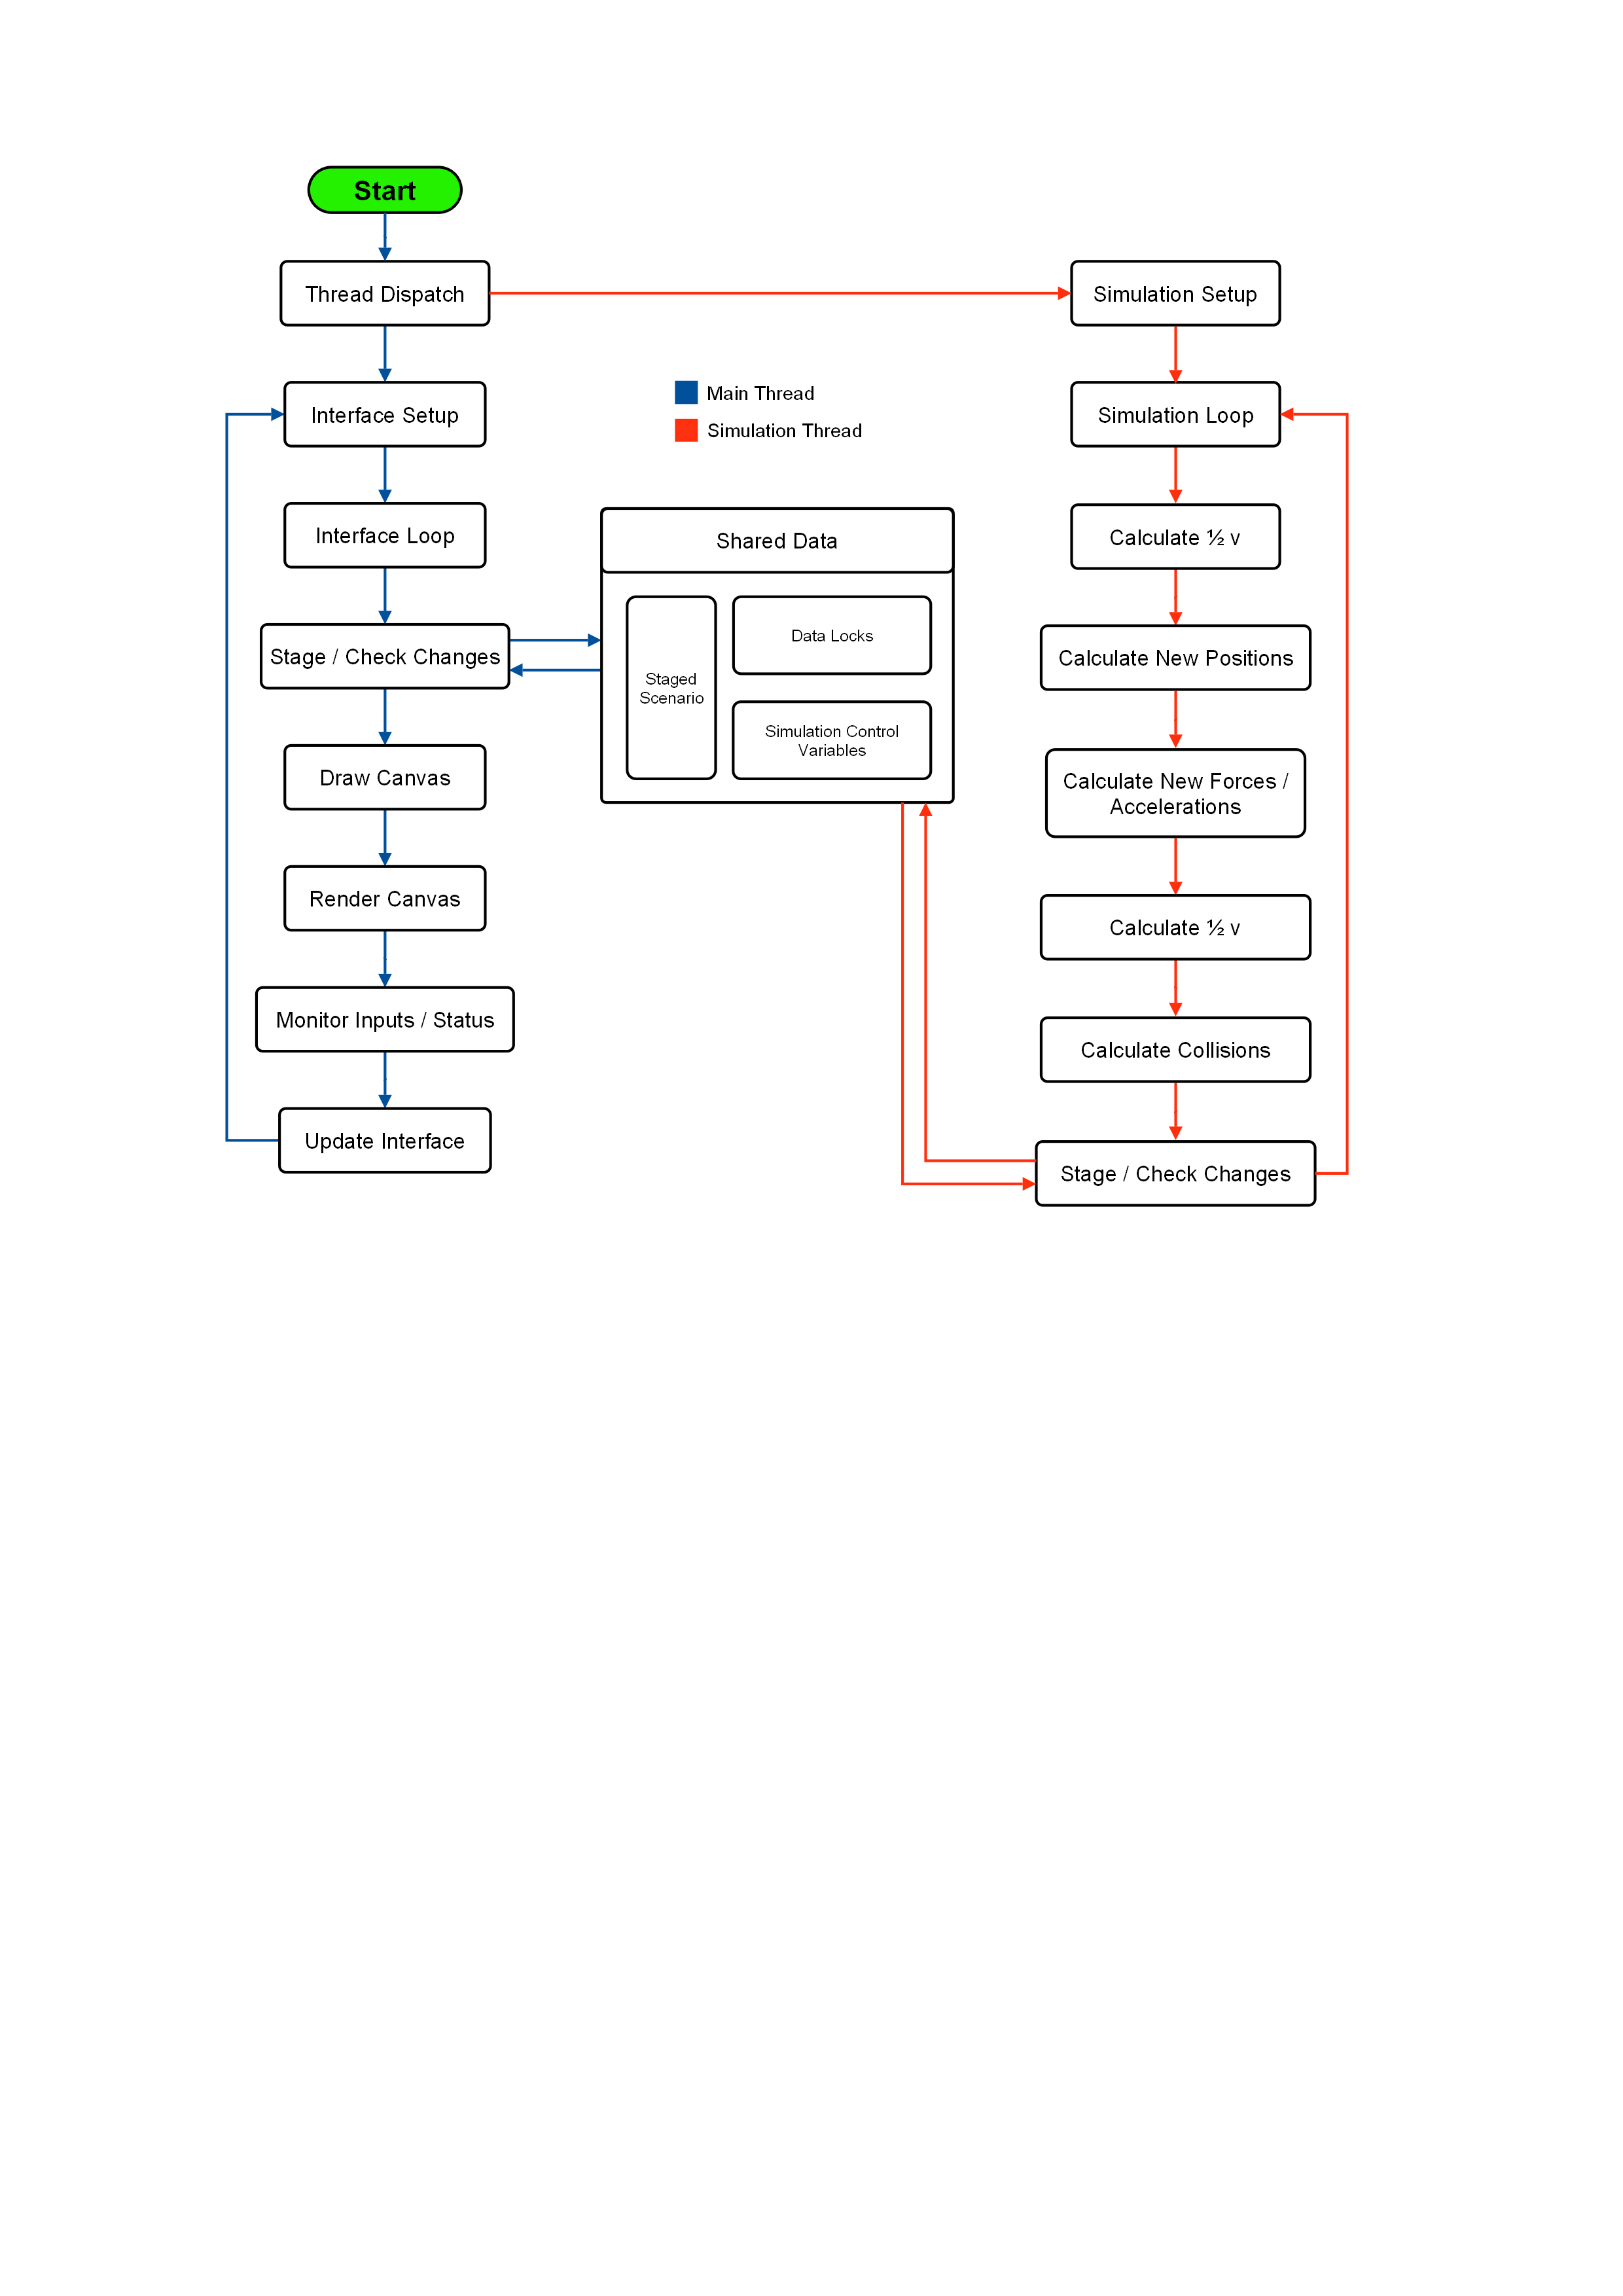
\includegraphics[scale=1]{../img/flowchartNew.png} 
  \caption{Improved Flowchart}
\end{figure}

\pagebreak
\subsection{Code Listing}
\subsubsection{main.cpp - Root Implementation}
\texttt{\lstinputlisting{../../../exo/src/main.cpp}} 
\pagebreak
\subsubsection{body.hpp - Interface}
\texttt{\lstinputlisting{../../../exo/include/body.hpp}} 
\pagebreak
\subsubsection{body.cpp - Implementation}
\texttt{\lstinputlisting{../../../exo/src/body.cpp}} 
\pagebreak
\subsubsection{scenario.hpp - Interface}
\texttt{\lstinputlisting{../../../exo/include/scenario.hpp}} 
\pagebreak
\subsubsection{scenario.cpp - Implementation}
\texttt{\lstinputlisting{../../../exo/src/scenario.cpp}} 
\subsubsection{render.hpp - Interface}
\texttt{\lstinputlisting{../../../exo/include/render.hpp}} 
\pagebreak
\subsubsection{render.cpp - Implementation}
\texttt{\lstinputlisting{../../../exo/src/render.cpp}} 
\pagebreak
\subsubsection{simulation.hpp - Interface}
\texttt{\lstinputlisting{../../../exo/include/simulation.hpp}} 
\pagebreak
\subsubsection{simulation.cpp - Implementation}
\texttt{\lstinputlisting{../../../exo/src/simulation.cpp}} 
\pagebreak
\subsubsection{shared.hpp - Interface}
\texttt{\lstinputlisting{../../../exo/include/shared.hpp}} 
\pagebreak
\subsubsection{shared.cpp - Implementation}
\texttt{\lstinputlisting{../../../exo/src/shared.cpp}} 
\pagebreak
\subsubsection{ui.hpp - Interface}
\texttt{\lstinputlisting{../../../exo/include/ui.hpp}} 
\pagebreak
\subsubsection{ui.cpp - Implementation}
\texttt{\lstinputlisting{../../../exo/src/ui.cpp}} 
\begin{sidewaysfigure}
  \subsubsection{Final Interface}
  \centering
  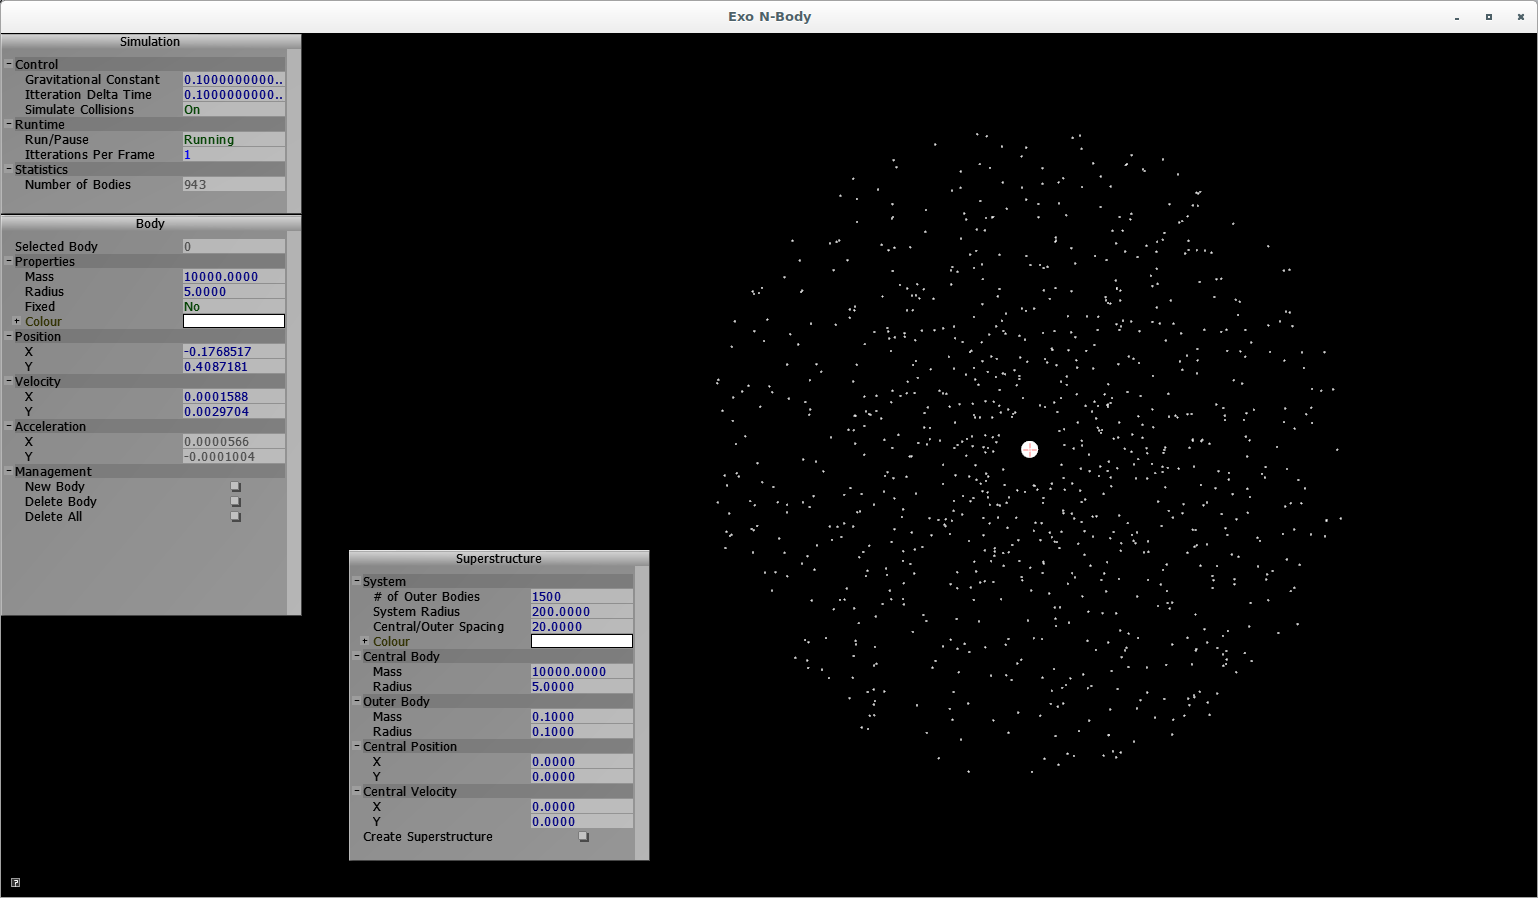
\includegraphics[width=\textwidth]{../img/finalInterface.png} 
  \caption{Full View of Complete Interface}
\end{sidewaysfigure}
\pagebreak

\begin{figure}[h]
  \centering
  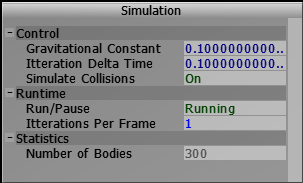
\includegraphics[scale=0.7]{../img/simUI.png} 
  \caption{Simulation Control UI}
\end{figure}

\begin{figure}[h]
  \centering
  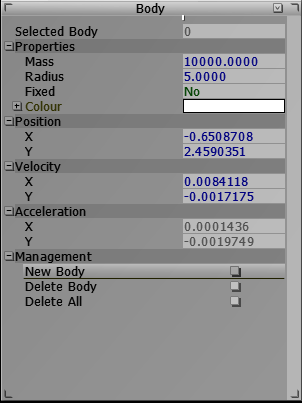
\includegraphics[scale=0.6]{../img/bodyUI.png} 
  \caption{Body Control UI}
\end{figure}

\begin{figure}[ht]
  \centering
  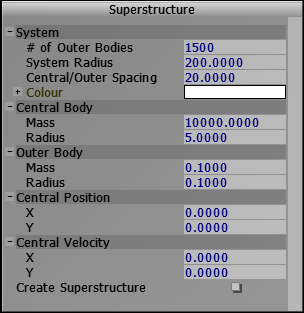
\includegraphics[scale=0.7]{../img/superstructureUI.png} 
  \caption{Superstructure Creation UI}
\end{figure}

\pagebreak